\section{Relational Manipulation Programs}
\label{sec:relational_programs}

We now define relational primitives, their composition into task-level strategies, and their instantiation in novel scenes.

\subsection{Primitives as Local Trajectory-Optimization Programs}
\label{sec:relational_primitives}
A primitive is a reusable behavior for realizing an object-level motion effect, such as pushing for a displacement or flipping for an angle. We represent a primitive as a local relational trajectory-optimization program
\begin{equation*}
    P_i=(G_i,C_i,\Psi_i,\rho_i,J_i)\in\mathcal{P}.
\end{equation*}
Here, $G_i$ is a semantic, object-centric description of the intended effect; $C_i$ is the relational interface; $\Psi_i$ is the verifiable success condition; $\rho_i$ is the geometry resolver; and $J_i$ is the optimization cost. Together, these components specify how the primitive is instantiated, optimized, and verified in a specific scene. A primitive is therefore neither a fixed trajectory nor a black-box policy. Table~\ref{tab:flip_primitive} illustrates each component for flipping an object against a fixture.

\begin{table}[t]
    \caption{\textbf{Object-centric trajectory optimization program for flipping.}}
    \label{tab:flip_primitive}
    \begin{adjustbox}{width=\columnwidth}
    \centering
    \setlength{\tabcolsep}{2pt}
    \begin{tabular}{@{}>{\raggedright\arraybackslash}p{0.37\columnwidth}
                        >{\raggedright\arraybackslash}p{1.13\columnwidth}@{}}
        \toprule
        \textbf{Component} & \textbf{Content} \\
        \midrule
        Semantic goal $G_i$
            & Flip the target against the vertical fixture for a specific angle. \\
        \rowcolor{black!5}
        Relational contract $C_i$
            & Semantic roles $\mathbf{r}_i$: target, support plane, fixture, and pusher.
              Relations $\Gamma_i$: the target rests on the support plane, and the fixture
              exposes a reachable vertical face. Effect parameter $\mathbf{q}_i$: flipping angle.\\
        Success predicate $\Psi_i$
            & Check that the achieved rotation matches the flipping angle and that the
              target remains supported, near the fixture, and settled. \\
        \rowcolor{black!5}
        Geometry resolver $\rho_i$
            & At each rollout state, derive the support plane, fixture face,
              pivot axis, target faces, dimensions, and clearances. \\
        Final cost $J_i^{\mathrm{f}}$
            & Penalize terminal rotation error relative to the flipping angle, support
              and fixture gaps, and terminal velocity. \\
        \rowcolor{black!5}
        Progress cost $J_i^{\mathrm{p}}$
            & Encourage rotation and pusher proximity while discouraging
              backtracking and irregular motion. \\
        \bottomrule
    \end{tabular}
    \end{adjustbox}
    \vspace{-0.3in}
\end{table}

\xhdr{Relational interface.}
We write the primitive interface as
\begin{equation*}
    C_i=(\mathbf{r}_i,\Gamma_i,\mathbf{q}_i).
\end{equation*}
The declarations $\mathbf{r}_i$ and $\mathbf{q}_i$ specify the semantic scene roles and typed effect-parameter slots required by $P_i$, while $\Gamma_i$ specifies the relations among the roles. An invocation supplies runtime arguments $(b_i,g_i)$ satisfying
\begin{equation*}
    b_i\in\operatorname{Bind}_E(\mathbf{r}_i,\Gamma_i),
    \qquad
    g_i\in\operatorname{Val}(\mathbf{q}_i).
\end{equation*}
Here, $\operatorname{Bind}_E(\mathbf{r}_i,\Gamma_i)$ denotes the type-compatible assignments of scene entities from the environment $E$ to $\mathbf{r}_i$ that satisfy $\Gamma_i$, and $\operatorname{Val}(\mathbf{q}_i)$ denotes the values matching the types declared by $\mathbf{q}_i$. In the flipping example (Table~\ref{tab:flip_primitive}), $b_i$ binds the target, support plane, fixture, and pusher to scene entities, while $g_i$ supplies the requested angle. Scene-dependent geometry remains internal to the primitive and is resolved by $\rho_i$ at execution time.

\xhdr{Geometry resolver.}
Let $\mathcal{X}(E)$ be the state space of environment $E$. At each state $x_t\in\mathcal{X}(E)$ along a rollout, the geometry resolver computes
\begin{equation*}
    \phi_{i,t} = \rho_i(E,x_t,b_i), \qquad t=0,\ldots,T,
\end{equation*}
where $\phi_{i,t}$ collects the geometric features at time $t$.

\xhdr{Success predicate.}
For a terminal state $x_T\in\mathcal{X}(E)$, the predicate $\Psi_i(E,x_T;g_i,\phi_{i,T})\in\{0,1\}$ provides an executable interpretation of $G_i$. It evaluates the achieved object relations and requested effect, yielding an unambiguous signal for verification. 

\xhdr{Optimization cost.}
For a simulated trajectory $\tau=(x_0,\ldots,x_T)$ in environment $E$, where $x_t\in\mathcal{X}(E)$, the primitive cost is
\begin{equation*}
    \begin{aligned}
        J_i(E,\tau;g_i,\phi_{i,0:T})
        = J_i^{\mathrm{f}}(E,x_T;g_i,\phi_{i,T}) 
        + \lambda_i J_i^{\mathrm{p}}(E,\tau;g_i,\phi_{i,0:T}).
    \end{aligned}
\end{equation*}
Here, $J_i^{\mathrm{f}}$ is the final cost, which measures how far $x_T$ is from the effect encoded by $G_i$; $J_i^{\mathrm{p}}$ is the progress cost, which may depend on the full trajectory and guides the optimizer through contact-rich interaction heuristics; and $\lambda_i\geq 0$ is a constant. The coding agent proposes the heuristics by reasoning about the visual human demonstration.

During primitive construction, the agent also proposes an initialization heuristic based on the resolved geometry and requested effect. The heuristic provides a plausible interaction trajectory from which to begin the search. Let $z$ parameterize a candidate robot motion, let $\tau(z)=\operatorname{Rollout}_E(x_0,z)$ denote its simulated state trajectory from $x_0$ in environment $E$, and let $\phi_{i,0:T}(z)$ be the feature sequence resolved along that trajectory. The executable trajectory is obtained as
\begin{equation*}
    z_i^\star
    = \arg\min_z
    J_i\!\left(E,\tau(z);g_i,\phi_{i,0:T}(z)\right).
\end{equation*}
We solve this trajectory-optimization problem with the Cross-Entropy Method (CEM)~\cite{deboer2005tutorial}, a sampling-based optimizer. We use CEM because it is gradient-free, allowing us to optimize robot motions without differentiating through the contact-rich simulation. The primitive thereby adapts its motion to the object pose, size, geometry, physical properties, and requested effect.

\subsection{Strategies as Primitive Composition by Constraints}
\label{sec:relational_strategy}

\begin{figure}[t]
    \centering
    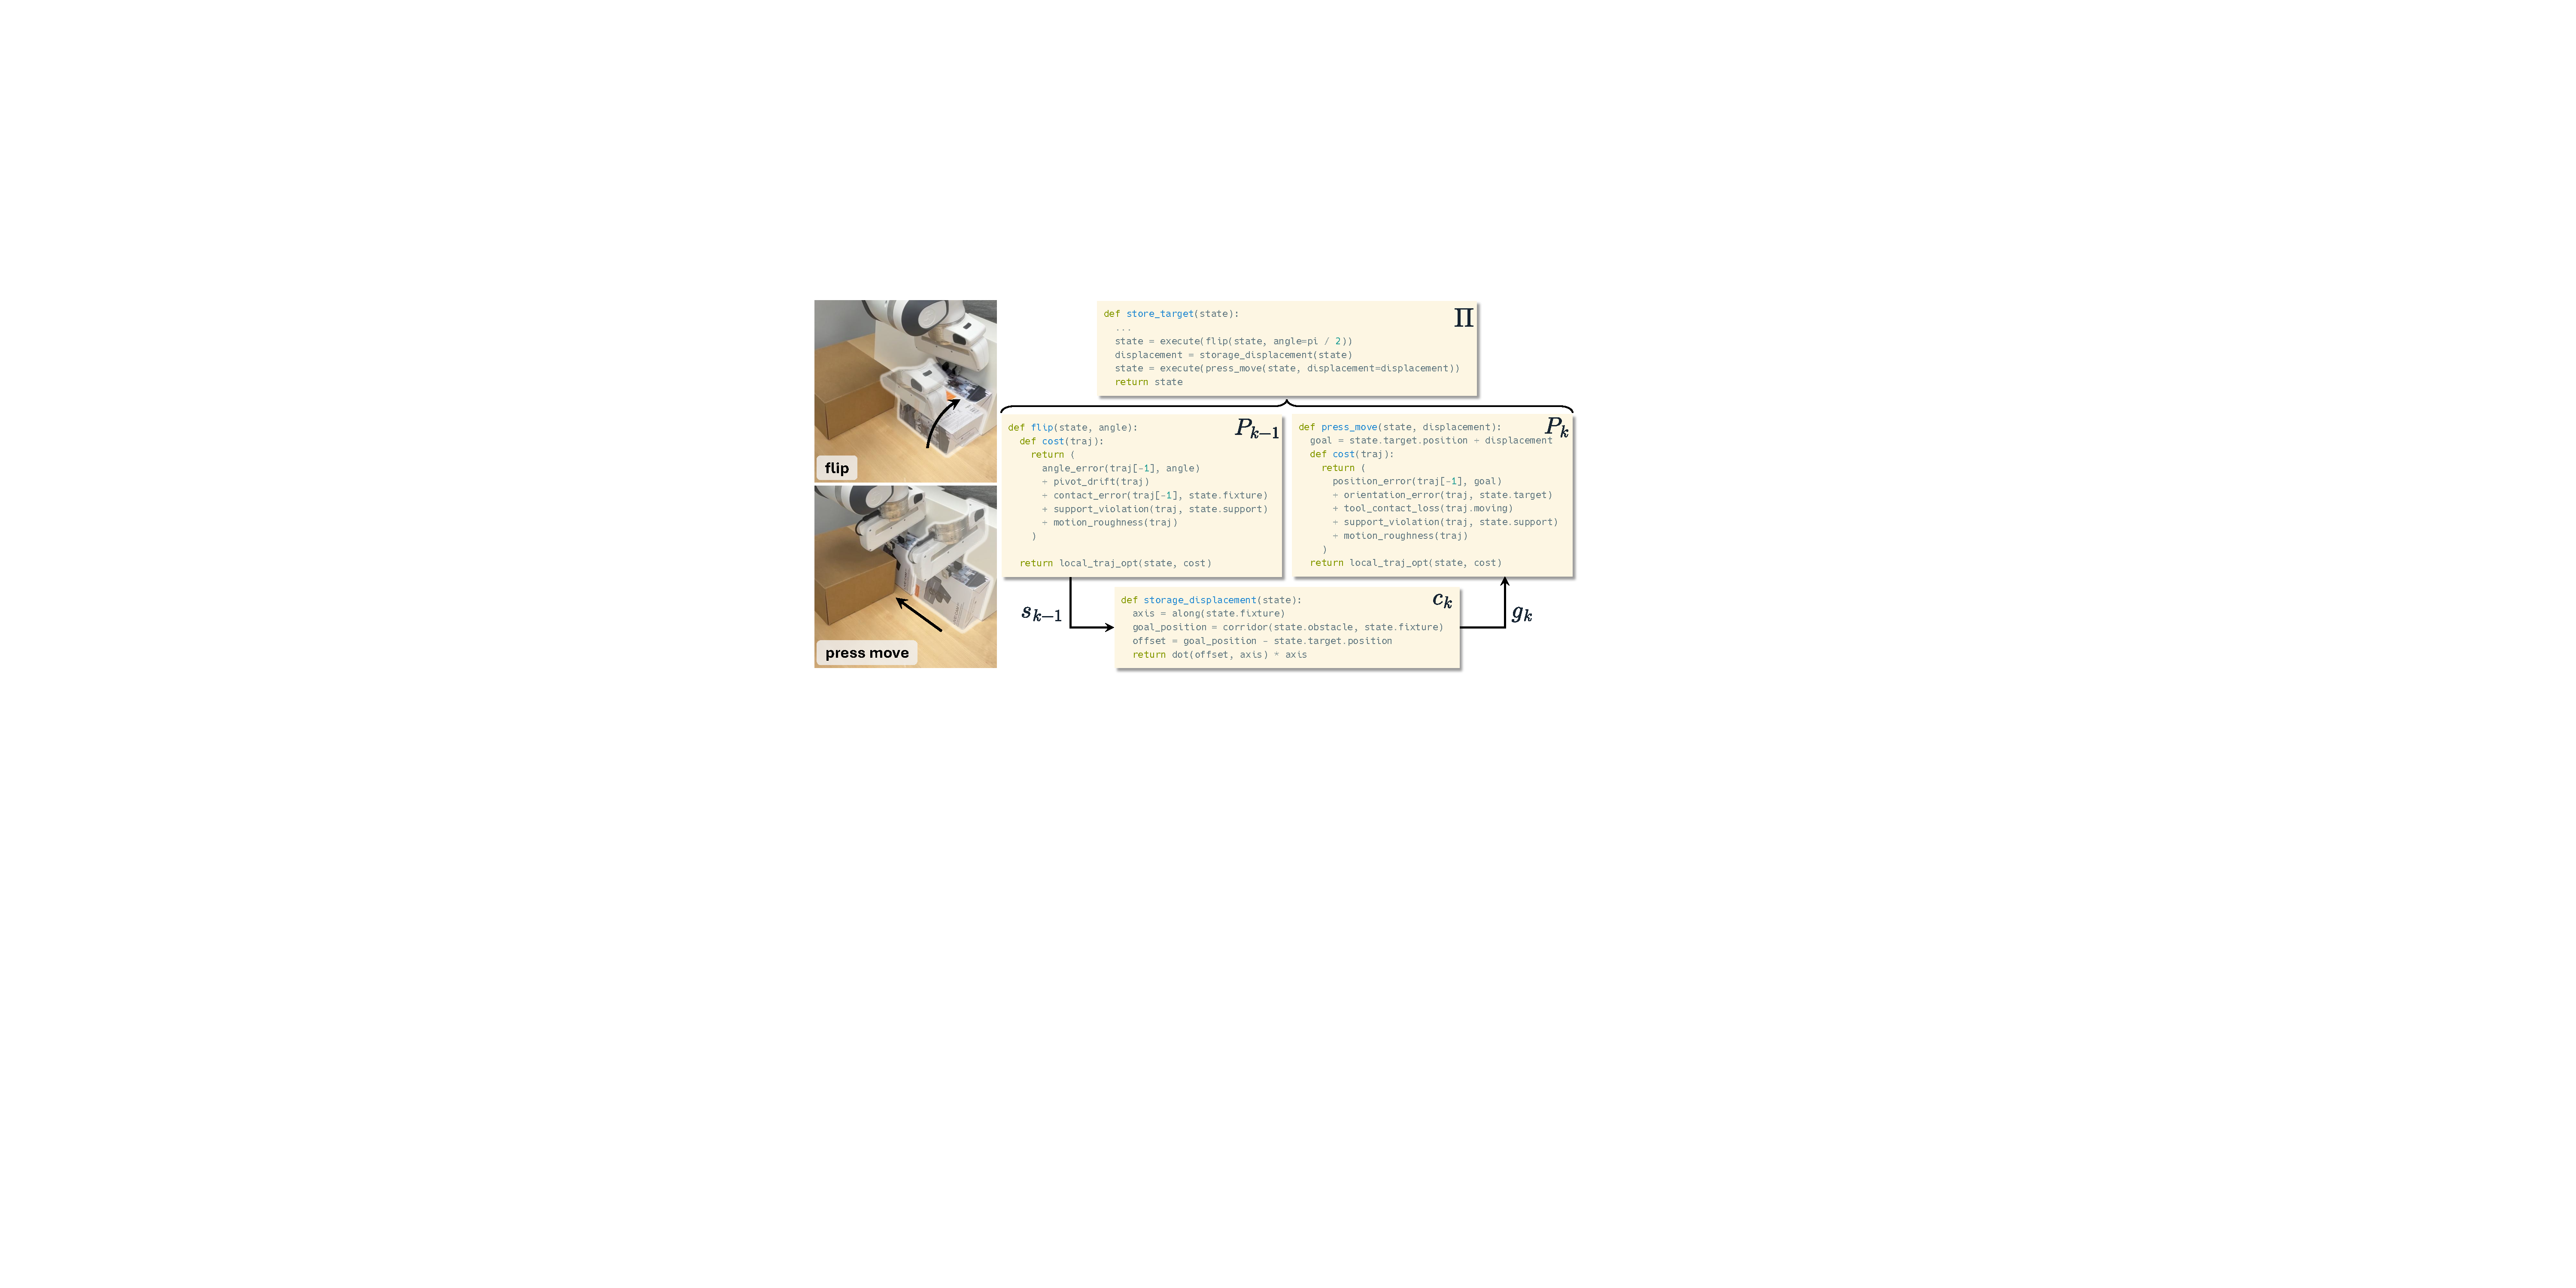
\includegraphics[width=\linewidth]{figures/program.pdf}
    \caption{\textbf{Composing primitives by relational constraints.}}
    \label{fig:program}
    \vspace{-0.3in}
\end{figure}

Suppose we have a library of primitives $\mathcal{P}$, where each $P_i \in \mathcal{P}$ realizes an object-level motion effect. A strategy $\Pi$ is a reusable task-level program that composes these primitives to accomplish an overall task. It specifies the sequence of primitives to invoke, how task roles map to each primitive, and how the requested effect of each invocation is determined:
\begin{equation*}
    \Pi
    = \left(G_\Pi,C_\Pi,\Psi_\Pi,
      \left\langle(P_{i_k},m_k,c_k)\right\rangle_{k=1}^{K}\right),
\end{equation*}
where $G_\Pi$ describes the overall task goal and $\Psi_\Pi$ evaluates its final outcome.

\xhdr{Strategy interface.}
A strategy exposes semantic roles and their required relations,
\begin{equation*}
    C_\Pi=(\mathbf{r}_\Pi,\Gamma_\Pi).
\end{equation*}
To invoke the strategy, a role binding $b\in\operatorname{Bind}_E(\mathbf{r}_\Pi,\Gamma_\Pi)$ assigns an entity to each strategy role while satisfying $\Gamma_\Pi$. Primitive effect parameters are not exposed through $C_\Pi$; instead, they are derived inside the strategy during execution.

\xhdr{Primitive Composition by Constraints.}
A strategy consists of $K$ phases, each represented by a tuple $(P_{i_k},m_k,c_k)$, where $P_{i_k} \in \mathcal{P}$ is a primitive, $m_k$ is a role map, and $c_k$ is a connecting constraint. For the invoked primitive $P_{i_k}$, $m_k$ produces a role binding $b_k$ that fills the role declarations $\mathbf{r}_{i_k}$, while $c_k$ produces an effect argument $g_k$ that fills the parameter declarations $\mathbf{q}_{i_k}$. The connecting constraint declaratively specifies how phase $k$ depends on the outcome of phase $k-1$ and is evaluated just in time at the beginning of phase $k$:
\begin{equation*}
    \begin{aligned}
        b_k&=m_k(b)
            \in\operatorname{Bind}_E(\mathbf{r}_{i_k},\Gamma_{i_k}),\\
        g_k&=c_k(E,s_{k-1},b)
            \in\operatorname{Val}(\mathbf{q}_{i_k}),
    \end{aligned}
\end{equation*}
where $s_{k-1}\in\mathcal{X}(E)$ denotes the environment state after the execution of phase $k-1$. The phase is then executed as
\begin{equation*}
    s_k=\operatorname{Exec}\!\left(
        P_{i_k};E,s_{k-1},g_k,b_k\right).
\end{equation*}
Here, $\operatorname{Exec}$ solves the local trajectory-optimization problem of $P_{i_k}$ and executes the optimized trajectory.

For example, Figure~\ref{fig:program} shows a \textit{press move} following a \textit{flip}. The role map $m_k$ maps the strategy's target object, supporting surface, and tool roles to the corresponding roles of the \textit{press-move} primitive, producing $b_k$. The connecting constraint $c_k$ determines the goal position from the relation between the brown obstacle and the white fixture. Using the target object's current position in the post-flip state $s_{k-1}$, it computes the displacement toward this goal along the fixture axis, producing the effect argument $g_k$ for the \textit{press move} primitive.

\subsection{Strategy Instantiation in Novel Scenes}
\label{sec:novel_instantiation}

To deploy a strategy in a novel scene, we only need to provide a semantic binding. Given a novel scene $E^\star$ and instruction $l^\star$, RAPID uses a coding agent to rapidly generate a semantic binding $b^\star \in\operatorname{Bind}_{E^\star}(\mathbf{r}_\Pi,\Gamma_\Pi)$ that assigns scene entities to the semantic roles exposed by the strategy interface.Since this step only associates the exposed semantic roles with scene entities, it is lightweight and incurs little deployment overhead. At phase $k$, the strategy derives the primitive binding and effect argument automatically. 

Throughout this process, the strategy program $\Pi$ and the referenced primitives remain frozen. Generalization therefore arises from the relational program representation, together with the adaptation of trajectory optimization to the geometry and physical properties of the new scene.
